\documentclass{article}
\usepackage[main]{template/neurips_2026}
\usepackage[utf8]{inputenc}
\usepackage[T1]{fontenc}
\usepackage{amsmath,amssymb}
\usepackage{graphicx}
\usepackage{booktabs}
\usepackage{microtype}
\usepackage{xcolor}
\usepackage{url}
\usepackage{xurl}
\usepackage{hyperref}
\hypersetup{colorlinks=true,citecolor=blue,linkcolor=blue,urlcolor=blue}
\newcommand{\MainSeconds}{42.0}
\newcommand{\ZeroUpper}{3.7}
\newcommand{\MainFitCount}{15032}
\newcommand{\AdjacentCount}{160}
\newcommand{\MaxGradient}{1.0e-08}

\newcommand{\R}{\mathbb{R}}
\newcommand{\sigmoid}{\sigma}
\newcommand{\editset}{\mathcal{S}}

\title{When Two Flips Suffice: Exposure and Estimator Dependence\\in Pairwise Leaderboard Audits}
\author{Anonymous Authors}

\begin{document}
\maketitle

\begin{abstract}
How should a small perturbation budget be interpreted in a pairwise leaderboard? We audit outcome reversals on fixed observed comparison schedules using sum-loss ridge Bradley--Terry fits. A frozen influence ordering proposes distinct decisive-row flips; full numerical refits verify whether the original runner-up exceeds the original leader. Across an Arena crowd snapshot, MT-Bench human and GPT-4 judgments, and three NBA seasons, sufficient budgets are respectively 2, 46, 61, 3, 4, and 8 rows. These are witness upper bounds, not minimum edit counts or robustness certificates. Reporting both dataset size and target-union exposure changes the scale of these budgets: the two Arena edits are 0.0035\% of all rows but 0.024\% of target exposure. Uniform and target-incident uniform controls each yield no reversals in 100 equal-budget trials per dataset; edge-matched random controls sometimes succeed. Exact ordered-cell matching retains a larger GPT-4 than human witness budget on a selected MT-Bench support, without identifying a causal judge effect. Crucially, Arena's leading pair is already weakly separated under empirical resampling, and removing ties reverses its order without edits. Fixed-target ridge and tie ablations therefore qualify any single fragility number. The contribution is a source-bounded, reproducible fixed-schedule audit with exposure accounting, controls, and estimator-conditional evidence, rather than a first demonstration of ranking vulnerability or refit-based sensitivity analysis.
\end{abstract}

\section{Introduction}
\label{sec:introduction}
Pairwise leaderboards turn heterogeneous comparisons into a compact ordering. The first two entries may influence model choice even when their fitted strengths are nearly equal. A useful audit should ask not only whether a selected set of changed observations reverses that ordering, but also what constitutes an observation, which estimator is being perturbed, and what denominator makes the change interpretable. Two changed rows in a large comparison graph can represent a different intervention from two changed rows concentrated on a sparsely observed target pair.

Existing work already establishes that rankings can be sensitive to small, directed changes. Most directly, \citet{huang2025dropping} audit influential preference deletions on Arena and MT-Bench, verify candidate ranking changes by full refits, compare evaluation designs and judges, and examine exposure and score gaps. Influence-based deletion sensitivity with refit verification also predates that study \citep{broderick2020automatic}. New-vote manipulation is another established threat model \citep{min2025improving}. Thus neither small-data sensitivity, cross-design comparisons, nor exact numerical refitting alone is the contribution here.

We instead study a bounded intervention: reverse selected decisive outcomes while retaining every original comparison, participant, and row weight. This holds the observed comparison schedule fixed, unlike deletion or appending new battles. We pair the resulting finite-flip witnesses with explicit target-exposure accounting, equal-budget random controls, matched-support checks, and an NBA outcome-domain comparison. The NBA analysis asks whether similar accounting issues appear outside preference judgments; it does not equate changing a recorded game outcome with correcting a human label.

A central limitation is visible before interpreting the smallest budget: a very small fitted margin can be sensitive both to label changes and to estimator conventions. Our Arena example is such a case. Its original leading pair retains a positive gap in only 110 of 200 empirical resamples, and removing ties reverses the original pair without any outcome flips. The headline two-flip result is therefore evidence about a specified estimator and weakly separated pair, not a demonstration that a clearly established population winner can be displaced by two realistic annotation errors.

The study makes three bounded contributions. First, it documents six refit-verified witnesses for distinct binary reversals on fixed observed schedules, reporting target identities, margins, dataset fractions, and target-union exposure fractions together. Second, it compares these witnesses with uniform, incident, direction-beneficial, and edge-matched random controls, then examines ordered-cell matched MT-Bench judgments and genuinely distinct size-controlled Arena subsets. Third, it freezes target identities across estimator ablations and separates finite-sample edit sensitivity from selected-target empirical resampling. No new theory, globally optimal attack algorithm, or state-of-the-art advantage is claimed.

All conclusions concern the empirical datasets and fitting conventions audited here. The fits use all observed rows, not a supervised training/test split, and do not reproduce Arena's production ranking pipeline. Our literature positioning is limited to five authorized, actually consulted sources; it is not an exhaustive novelty assessment.

\section{Related work}
\label{sec:related}
\paragraph{Preference evaluation and leaderboard estimation.}
\citet{zheng2023judging} introduce MT-Bench and examine human/model judging, including position bias and order-inconsistent judgments. Their results motivate preserving the exported judgment unit and reporting tie treatment rather than treating model verdicts as independent, error-free calls. \citet{chiang2024chatbot} describe Arena's nonuniform comparison sampling, statistical estimation, uncertainty, and inverse-probability weighting. Our unweighted empirical-design ridge fit uses neither unavailable sampling propensities nor production language filters. Exposure normalization of an edit budget is an accounting choice, not inverse-probability weighting of the fitted objective.

\paragraph{Deletion sensitivity and the closest audit.}
\citet{broderick2020automatic} linearize a smooth estimator's sensitivity to observation weights, select harmful deletions, and refit to obtain achieved changes. An achieved change lower-bounds maximum attainable sensitivity; equivalently, a successful edit set upper-bounds the unknown minimum budget for its endpoint. \citet{huang2025dropping} apply related ideas to BT top-$k$ membership, using full refits on influential deletions and comparisons across Arena, MT-Bench, and human/model judgments. They also inspect model appearances and gap associations. We do not characterize their work as ignoring exposure or lacking refit verification. Our narrower contrast is fixed-schedule outcome reversal, explicit exposure-scaled budget reporting and controls, plus estimator-conditional and NBA evidence. The same-estimator deletion comparator below is not a reproduction of their filtering, unregularized estimator, or published counts.

\paragraph{Outcome manipulation and threat-model boundaries.}
\citet{min2025improving} choose outcomes for newly encountered battles and append votes, including effects through comparisons not involving a target. Outcome choice and indirect effects are therefore not new ideas. We allow retrospective access to the observed labels and estimator and reverse existing decisive rows once each. This is an offline sensitivity intervention, not a demonstrated strategy for changing stored votes on a live platform. Within this source-bounded reading, the value of the audit is its specified intervention and evidence trail, not a claim of priority over all ranking-robustness methods.

\section{Method: a fixed-schedule finite-flip audit}
\label{sec:method}
\subsection{Estimator and intervention}
\label{sec:estimator}
For row $i$, let $u_i,v_i$ be its participants, $x_i=e_{u_i}-e_{v_i}\in\R^M$, and $y_i$ the outcome for $u_i$. Decisive outcomes are $0$ or $1$; retained ties are assigned $1/2$. With $N$ rows, we fit
\begin{equation}
\begin{aligned}
\hat\theta&=\arg\min_{\theta\in\R^M} L(\theta;y),\\
L(\theta;y)&=\sum_{i=1}^{N}\left[\log(1+\exp(x_i^\top\theta))-y_i x_i^\top\theta\right]\\
&\quad+\frac{\lambda}{2}\|\theta\|_2^2.
\end{aligned}
\label{eq:objective}
\end{equation}
This is a \emph{sum} loss with $\lambda=1$ in the primary audit. Positive ridge makes the objective strictly convex and coercive; its unique minimizer has centered participant scores. It also prevents separation from producing diverging estimates. These properties do not guarantee that the BT model describes the data-generating process. Appendix~\ref{app:derivation} supplies the elementary derivation and the home-covariate extension.

The primary targets are the original leader $a$ and runner-up $b$. Write $c=e_a-e_b$ and $\hat\Delta=c^\top\hat\theta>0$. An edit set $\editset$ contains distinct decisive rows, each changed once by $y_i\mapsto1-y_i$. Ties are never eligible. Every original pair, covariate, and weight is retained. After a full numerical refit, success is
\begin{equation}
\Delta(\editset)=c^\top\hat\theta(y^{\editset})<-\varepsilon,\qquad \varepsilon=10^{-7}.
\label{eq:event}
\end{equation}
This event implies the original leader is strictly dethroned, but does not require $b$ to become the new overall leader. It is not the minimum number of changes for \emph{any} top-one change. Exact numerical ties do not count as reversals.

\subsection{Local ordering and finite verification}
\label{sec:search}
We use a local approximation only to order candidate rows. At the fitted solution let $p_i=\sigmoid(x_i^\top\hat\theta)$ and
\begin{equation}
\begin{aligned}
H&=\sum_i p_i(1-p_i)x_i x_i^\top+\lambda I,\\
\delta y_i&=1-2y_i,\qquad B_i=-\delta y_i\,x_i^\top H^{-1}c.
\end{aligned}
\label{eq:benefit}
\end{equation}
Implicit differentiation gives the first-order margin change $\delta y_i c^\top H^{-1}x_i$; hence positive $B_i$ predicts a decrease in the leader's margin. This is not an approximation-error bound for a finite binary edit. In particular, no deletion robustness theorem is transferred to flips.

We sort decisive rows by decreasing positive benefit, using stable ordering and a numerical selection cutoff of $10^{-14}$. The ordering is frozen at the original fit. We refit prefixes at powers of two, capped at $\lfloor0.2N_{\rm dec}\rfloor$ decisive rows and the available positive-benefit list length. On finding a noncrossing/crossing bracket, bisection produces a verified neighboring transition. We refit both the reported prefix $k$ and $k-1$ and retain the row identifiers and margins.

The returned $k$ is a sufficient witness, \emph{not necessarily the first crossing even along this list}: the finite-refit margin need not be monotone. Powers-of-two probes can miss crossings that subsequently disappear, and beneficial joint edits may include rows excluded by the initial ordering. Thus a found $k$ upper-bounds the unknown minimum for Eq.~\eqref{eq:event}; an unsuccessful search leaves the question unresolved. Neither convergence of the optimizer nor verification of $k-1$ certifies combinatorial optimality.

\subsection{Exposure accounting and controls}
\label{sec:exposure}
Define target-union exposure and direct exposure as
\begin{equation}
\begin{aligned}
E_{ab}&=\sum_i\mathbf{1}\!\left[\{u_i,v_i\}\cap\{a,b\}\ne\varnothing\right],\\
D_{ab}&=\sum_i\mathbf{1}\!\left[\{u_i,v_i\}=\{a,b\}\right].
\end{aligned}
\label{eq:exposure}
\end{equation}
A direct comparison counts once, not twice, in $E_{ab}$. Both $N$ and $E_{ab}$ include retained ties, so neither is the decisive edit-pool size. We report $k$, $k/N$, and $k/E_{ab}$. The unrestricted search can select nonincident rows; generally $k/E_{ab}$ is an exposure-scaled \emph{total} cost, not the fraction of incident rows corrupted. All six primary witnesses happen to be entirely incident, making that latter interpretation valid for these six witnesses only.

At each dataset's witnessed $k$, we sample 100 control subsets without replacement within a trial: (i) uniform decisive rows; (ii) uniform target-incident decisive rows; (iii) target-incident decisive rows with positive initial benefit; and (iv) decisive rows matched to the witness's number of edits per unordered participant edge. The third control already uses target and outcome information. Edge matching fixes where edits occur, not their original outcome directions. These are randomized controls for a deterministic, data-adaptive witness, not interchangeable adversaries or population null hypotheses.

\section{Experiments}
\label{sec:experiments}
\subsection{Plan, data, and quality control}
\label{sec:data}
The pre-analysis plan was written before parsing and fitting; this remains an exploratory observational audit, not a preregistered causal comparison. Its stages were: reproduce and validate baseline fits; verify finite-flip witnesses and equal-budget controls; inspect resampling, matching, and estimator sensitivities; and generate reporting artifacts. Success signals were connected comparison graphs, converged fits, distinct decisive-row witnesses, repeated controls, and honest retention of failed or specification-sensitive comparisons. Ridge was specified rather than tuned for vulnerability.

\paragraph{Datasets and units.}
Arena supplies 57,477 crowd rows over 64 participants. All satisfy the specified threshold of at least 100 appearances, and no rows are removed. MT-Bench supplies 3,355 human judgments and 2,400 exported GPT-4 pair-result rows over six models. A GPT edit changes one exported result, \emph{not an individual underlying judging call}: the release does not expose separate reciprocal-call labels. Its 380 inconsistent results and 220 ordinary ties are both mapped to $1/2$ and held fixed in the primary audit. NBA seasons identified by \texttt{year\_id} 2013, 2014, and 2015 include regular-season and playoff games, with each season fitted separately. Duplicate team-side game records are removed by \texttt{\_iscopy==0}; one game is one row. A sports flip is a counterfactual recorded-outcome change, not evidence of a mistaken result.

Supplied snapshot hashes were verified. Preparation checks label validity, absence of missing mapped outcomes and self-comparisons, NBA game uniqueness, and observed undirected connectivity. All six primary graphs have one component. Arena's one-hot winner validation passes. Row identifiers are retained for reconstruction, and prompt/answer text is not needed in the processed edge lists. Appendix~\ref{app:data} reports tie counts, decisive-pool sizes, target names, and direct exposures. The observed test log records seven passing tests, including the regression that prevents numerical ties from counting as strict winner changes.

\paragraph{Fitting and evaluation protocol.}
All observed rows enter each baseline fit: there is no supervised train/validation/test partition, predictive accuracy metric, or out-of-sample generalization claim. Identical design rows are aggregated into sufficient statistics for optimization while edits retain original-row costs. Dense damped Newton fits target gradient infinity norm below $10^{-8}$ and reject returns above $10^{-7}$. Independent reconstruction from saved original row IDs verifies all six primary witnesses (\texttt{artifacts/witness\_verification.csv}). The corrected CPU-only main run took \MainSeconds{} seconds with single-thread BLAS; this is a container measurement, not a hardware-normalized benchmark. Appendix~\ref{app:reproduction} gives commands, pinned versions, hardware information and the isolated replay's memory measurement.

\subsection{Primary witnesses and denominator effects}
\label{sec:primary}
\begin{table}[t]
\centering
\caption{Primary fixed-schedule witnesses under sum-loss ridge BT ($\lambda=1$). $M$ is the participant count, $E_{ab}$ includes ties, and $\hat\Delta$ is the original leader--runner-up gap. Percentages use all rows or target-union exposure, not only decisive rows. Every $k$ is refit-verified, entirely target-incident, and an upper bound on the unknown minimum, not a certified minimum. Generated input: \texttt{paper/tables/main.tex}.}
\label{tab:main}
{\small\setlength{\tabcolsep}{4pt}\begin{tabular}{lrrrrrrr}
\toprule
Dataset & $N$ & $M$ & $E_{ab}$ & $\hat\Delta$ & $k$ & $100k/N$ & $100k/E_{ab}$ \\
\midrule
Arena crowd & 57,477 & 64 & 8,413 & 0.008 & 2 & 0.0035 & 0.024 \\
MT expert & 3,355 & 6 & 1,825 & 0.376 & 46 & 1.371 & 2.521 \\
MT GPT-4 & 2,400 & 6 & 1,440 & 0.809 & 61 & 2.542 & 4.236 \\
NBA 2013 & 1,314 & 30 & 199 & 0.219 & 3 & 0.228 & 1.508 \\
NBA 2014 & 1,319 & 30 & 196 & 0.279 & 4 & 0.303 & 2.041 \\
NBA 2015 & 1,311 & 30 & 193 & 0.693 & 8 & 0.610 & 4.145 \\
\bottomrule
\end{tabular}
}
\end{table}

Table~\ref{tab:main} establishes six sufficient budgets: 2, 46, 61, 3, 4, and 8. Full-precision Arena's gap is approximately 0.00813; its two-row reversal is 0.0035\% of all rows but 0.024\% of target exposure after rounding. The MT human and GPT-4 witnesses use 2.521\% and 4.236\% of target exposure. The NBA budgets fall between 1.508\% and 4.145\%. Changing the denominator does not change any witness; it makes explicit how much unrelated graph mass enters a global percentage. It can even reverse a descriptive cross-domain ordering: NBA 2015 has a smaller global fraction than MT human (0.610\% versus 1.371\%), but a larger exposure-scaled fraction (4.145\% versus 2.521\%). This is an accounting comparison of these witnesses, not a causal ranking of evaluation designs. Exposure scaling does not eliminate the Arena--MT difference or explain it causally.

\begin{figure}[t]
\centering
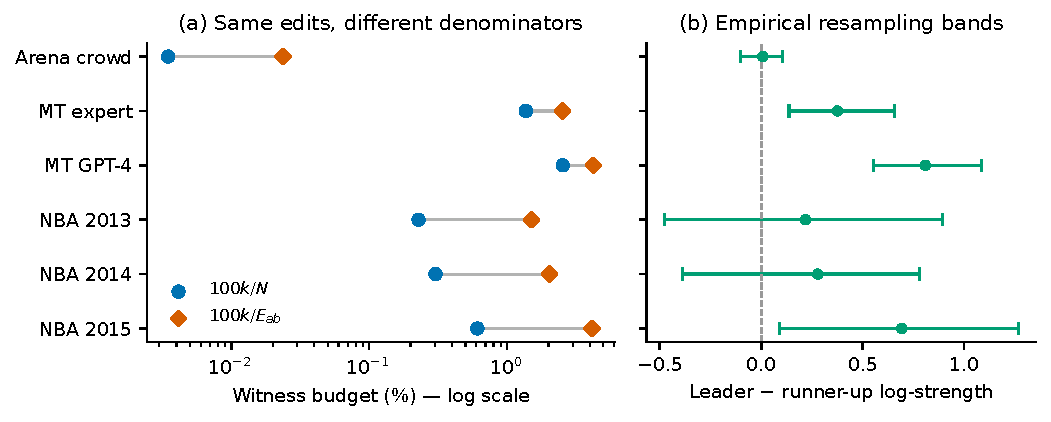
\includegraphics[width=\linewidth]{figures/budget_and_margin.pdf}
\caption{Accounting and separation must be read together. Left: the same verified edits as global and target-exposure percentages (log axis). Right: original gaps with 2.5th--97.5th percentile bands from 200 empirical row resamples for Arena/NBA or question-cluster resamples for MT. These change the comparison schedule and keep originally selected targets fixed; the bands are descriptive, not post-selection-valid or simultaneous confidence intervals and not uncertainty in a minimum flip budget. Source: \texttt{src/report.py}, \texttt{artifacts/baseline.csv}, and \texttt{artifacts/uncertainty.csv}.}
\label{fig:budget}
\end{figure}

Figure~\ref{fig:budget} shows why margin information belongs beside the budgets. Positive original-pair margins occur in 110/200 Arena resamples, 199/200 MT human, 200/200 MT GPT-4, and 155/200, 163/200, and 199/200 NBA resamples. In particular, the two-flip Arena witness accompanies substantial empirical resampling instability. These resamples do not preserve the original schedule and do not independently validate a population rank ordering.

\subsection{Equal-budget random comparisons}
\label{sec:controls}
\begin{table}[t]
\centering
\caption{Strict original-pair reversals at each dataset's witnessed $k$; 100 trials per control. Incident = incident-uniform; adverse = incident positive-benefit sampling. Edge matching fixes edit counts per unordered comparison edge, not outcome direction. Rates describe Monte Carlo variation conditional on these datasets and budgets. Generated input: \texttt{paper/tables/controls.tex}.}
\label{tab:controls}
{\small\begin{tabular}{lrrrr}
\toprule
Dataset & Uniform & Incident & Adverse & Edge-matched \\
\midrule
Arena crowd & 0/100 & 0/100 & 0/100 & 17/100 \\
MT expert & 0/100 & 0/100 & 0/100 & 0/100 \\
MT GPT-4 & 0/100 & 0/100 & 0/100 & 0/100 \\
NBA 2013 & 0/100 & 0/100 & 1/100 & 27/100 \\
NBA 2014 & 0/100 & 0/100 & 0/100 & 1/100 \\
NBA 2015 & 0/100 & 0/100 & 0/100 & 15/100 \\
\bottomrule
\end{tabular}
}
\end{table}

Uniform and incident-uniform controls yield zero successes throughout Table~\ref{tab:controls}. Zero successes do not mean impossibility: the two-sided 95\% Wilson upper endpoint is \ZeroUpper\% for 0/100. Edge-matched controls succeed in 17\%, 27\%, 1\%, and 15\% of Arena and NBA trials, respectively; both MT panels yield zero. Their pointwise Wilson intervals are, respectively, [10.9,25.5]\%, [19.3,36.4]\%, [0.2,5.4]\%, and [9.3,23.3]\%, rounded from \texttt{control\_summary.csv}. Incident-adverse sampling yields only one success, on NBA 2013.

The contrast supports a within-dataset targeting advantage over these specified controls, not a universal claim that random flips fail. Edge-matched successes show that locating edits on influential edges already explains part of the observed sensitivity. Conversely, fixing both edge and canonical original-outcome edit counts makes BT sufficient statistics identical by construction, so such replacements are an implementation-invariance check, not a new independent robustness experiment.

We report pointwise Monte Carlo intervals, not multiplicity-adjusted significance tests. No confirmatory hypothesis test or familywise claim is made across datasets, controls, budgets, or adjacent pairs. The deterministic witness itself needs no sampling error bar conditional on the supplied data and algorithm; its limitation is search incompleteness, not Monte Carlo uncertainty. Appendix~\ref{app:uncertainty} provides the interval formula, descriptive bootstrap table, and supplementary dose responses.

\subsection{Matched support and size/cohort checks}
\label{sec:matching}
\begin{table}[t]
\centering
\caption{Descriptive matching checks. MT uses the same 1,232 ordered question/model-pair/turn cells; 20 human runs vary the selected judge row per cell, whereas GPT is evaluated once. Arena uses 20 distinct 2,400-row subsets of a post-selected top-six pool, not MT's model cohort. Min/median/max are observed summaries, not confidence intervals. Generated input: \texttt{paper/tables/matched.tex}.}
\label{tab:matched}
{\small\setlength{\tabcolsep}{4pt}\begin{tabular}{lrrrr}
\toprule
Cohort & Runs & $N$ & $k$: min/med/max & $100k/E$: min/med/max \\
\midrule
MT expert matched & 20 & 1232 & 14/16.5/21 & 1.97/2.32/2.95 \\
MT GPT-4 matched & 1 & 1232 & 33/33/33 & 4.64/4.64/4.64 \\
Arena top-six (N=2400) & 20 & 2400 & 2/6/14 & 0.12/0.35/0.80 \\
\bottomrule
\end{tabular}
}
\end{table}

Exact MT matching intersects 1,232 ordered cells from 2,396 human and 2,400 GPT cells. For each seed, one observed human judgment is sampled per cell, preserving the decisive-row edit interpretation; GPT contributes its single matching exported result. This is an order-selected support: reverse-presentation cells outside the exact intersection are excluded. On this support, GPT's sufficient budget is 33 versus human budgets 14--21, with median 16.5 (Table~\ref{tab:matched}). The exposure-scaled GPT budget is 4.64\% versus a human median 2.32\%. The median human gap is 0.325 versus GPT's 0.819, so margin differences remain a plausible contributor. Twenty judge-choice seeds are not twenty independent datasets, and the comparison does not identify judge quality or a causal human-versus-model effect.

The Arena size check samples 2,400 rows without replacement from the 3,222-row induced pool of its full-fit top six participants. The current protocol records 20 distinct selected-row-set hashes; budgets range from 2 to 14, with median 6. The earlier attempt to match 3,355 rows exceeded this pool and selected the entire pool repeatedly; those obsolete pseudo-replicates are excluded. The corrected check shows that low budgets are not restricted to the full 57,477-row fit, but it changes participants, targets, margins, and relative ridge strength. It neither matches MT's participants nor isolates an evaluation-design effect.

\subsection{Estimator sensitivity and method comparisons}
\label{sec:sensitivity}
Fixed-target checks retain each primary pair's identities rather than selecting a new pair after every estimator change. Arena's witnessed budget is 1, 2, and 11 at ridge 0.1, 1, and 10. Removing ties already reverses the original Arena pair ($k=0$); this is a specification change, not a zero-cost attack on the original data. MT human's budget is 42 without ties, versus 46 with half ties. GPT's is 40 after removing all ties or 47 after excluding only inconsistent rows, versus 61 in the primary fit. NBA budgets remain 3, 4, and 8 under the tested ridge values and home adjustment. The home coefficient is penalized by the same ridge. Appendix~\ref{app:ablations} includes the full generated table and statuses.

Sequential relinearization and refitting after each selected flip gives the same budgets as the frozen ordering in all six primary panels. This is a negative result for a proposed search improvement on these instances, not evidence of global optimality. Static deletion under the same estimator and original targets yields sufficient witnesses of 3, 92, 144, 5, 7, and 16 deletions (Appendix~\ref{app:comparators}). Deletion and reversal are different interventions with different finite changes per row, so these counts do not establish algorithmic superiority or reproduce prior published deletion counts. Linear predictions also underestimate the verified MT budgets; full refits are consequential rather than ceremonial.

\section{Discussion and limitations}
\label{sec:discussion}
\paragraph{What the evidence supports.}
The audit supplies finite datasets on which specified small edit sets reverse an original leading pair, plus controls that make the edit location and direction interpretable. Exposure scaling prevents a large population of unrelated comparisons from being the only denominator. Neither the normalization nor matching makes the six panels exchangeable. Participants, prompts, judge populations, tie fractions, gaps, schedule balance, and outcome units differ. A fixed penalty in a sum loss also has different relative strength across sample sizes.

\paragraph{What remains unresolved.}
A near tie is intrinsically easier to reverse, and the Arena result is particularly estimator-dependent. The local ordering can miss better or transiently successful sets, so unsuccessful searches cannot certify stability. The unrestricted design does not imply incident-only optimality merely because the primary witnesses are incident. Empirical row resampling treats Arena votes and NBA games as its sampling units without modeling all user, time, team, or schedule dependence; MT question clustering does not capture every annotator dependence. Selected targets and overlapping subsets preclude interpreting percentile bands or seed ranges as independent, post-selection-valid population uncertainty. Adjacent-pair patterns are descriptive, not corrected significance findings.

\paragraph{Scope and practical interpretation.}
These are unweighted, regularized empirical fits, not official production Arena ranks or estimates corrected for unobserved propensities and language filtering. No label-correctness adjudication is performed. The ability to edit exported results offline does not establish real attacker access, plausibility, or the number of underlying GPT calls needed. NBA flips are hypothetical perturbations, not claims about game integrity. We have not demonstrated a defense, a real-world attack, or a causal advantage of one evaluation design. Future audits should report units, margins, target exposures, and estimator sensitivity before reducing fragility to a single percentage.

\paragraph{Responsible use and assistance.}
The study reuses public secondary data and recruits no people, solicits no votes, and alters no live service. Processed edge lists omit prompt/answer text; raw data are not bundled. Positive uses include transparent uncertainty communication and targeted audit design; misuse could include vote manipulation or selectively publicizing fragile ranks to mislead users. We provide offline evidence, not a live-deployment recipe or a tested mitigation; original-asset attribution and privacy constraints still apply. Appendix~\ref{app:ethics} discusses secondary-data ethics, incomplete compliance checks, release limitations, and LLM assistance beyond prose editing.

\section{Conclusion}
\label{sec:conclusion}
Two flips suffice for one specified Arena leading pair, while larger budgets are witnessed on MT-Bench and small game-count budgets on three NBA seasons. These are estimator- and target-conditional witnesses, not minima or statements of label error. Their interpretation changes when exposure, near-tie resampling behavior, controls, and tie/ridge conventions are reported together. The useful output is an auditable collection of finite reversals and limitations, rather than a universal vulnerability rate, a robustness certificate, or an exhaustive novelty claim.

% Main content ends here. Compile and inspect the actual page boundary before submission.
\label{main-text-end}
\clearpage
\bibliographystyle{plainnat}
\bibliography{references}
\clearpage
\appendix
% Included by main.tex after \appendix; not a standalone document.
\section{Objective, derivatives, and interpretation}
\label{app:derivation}
This appendix derives the algebra used for candidate ordering. It introduces no new robustness theorem, approximation guarantee, or promise of an exact minimum-budget solver. Assumptions are finite fixed design vectors, outcomes in $[0,1]$, positive ridge $\lambda$, and the sum-loss objective in Eq.~\eqref{eq:objective}. Binary reversals additionally require distinct selected rows with original outcomes in $\{0,1\}$.

\subsection{Existence, uniqueness, and centering}
Each logistic contribution in Eq.~\eqref{eq:objective} is nonnegative for $y_i\in[0,1]$. Therefore $L(\theta;y)\geq\lambda\|\theta\|_2^2/2$, making the continuous objective coercive. A finite minimizer exists. With $p_i=\sigmoid(x_i^\top\theta)$,
\begin{equation}
\nabla L=\sum_i x_i(p_i-y_i)+\lambda\theta,\qquad
\nabla^2 L=\sum_i p_i(1-p_i)x_i x_i^\top+\lambda I\succeq\lambda I.
\label{eq:gradient}
\end{equation}
Strict convexity gives uniqueness, regardless of undirected graph connectivity. Connectivity is still reported because it characterizes the observed comparison design; ridge does not create empirical comparisons between disconnected components. Since $\mathbf{1}^\top x_i=0$, the first-order condition implies $\lambda\mathbf{1}^\top\hat\theta=0$. Thus the unique participant vector is centered without fixing an arbitrary participant to zero. This differs from an unregularized reference-coded BT maximum-likelihood fit.

\subsection{Flip-benefit sign}
For a prospective edit of row $i$, consider the continuous path $y_i(t)=y_i+t\delta y_i$, with $\delta y_i=1-2y_i$, holding all other rows fixed. Positive ridge ensures a nonsingular Hessian along this path. Differentiating the first-order condition at $t=0$ gives
\begin{equation}
H\frac{d\hat\theta(t)}{dt}\bigg|_{t=0}-x_i\delta y_i=0,
\qquad
\frac{d(c^\top\hat\theta(t))}{dt}\bigg|_{t=0}
=\delta y_i c^\top H^{-1}x_i.
\label{eq:implicit}
\end{equation}
Negating this derivative yields $B_i$ in Eq.~\eqref{eq:benefit}. A positive score predicts a decrease of the leader-minus-runner-up gap. For multiple edits the linear prediction is $\hat\Delta-\sum_{i\in\editset}B_i$; it neglects curvature changes. The path calculation is exact as a derivative, not as a finite-flip equality. Reported successes always use the refitted objective, not this prediction.

\subsection{Sufficient statistics and physical-row accounting}
Choose a canonical orientation for each unordered participant edge $e$, with vector $x_e$. Let $s_i=+1$ if row $i$ agrees with that orientation and $-1$ otherwise, and set $\tilde y_i=y_i$ or $1-y_i$, respectively. The aggregate objective is
\begin{equation}
\begin{aligned}
L(\theta)&=\sum_e\left[n_e\log(1+\exp(x_e^\top\theta))-w_e x_e^\top\theta\right]
+\frac{\lambda}{2}\|\theta\|_2^2,\\
n_e&=\sum_{i:e(i)=e}1,\qquad w_e=\sum_{i:e(i)=e}\tilde y_i.
\end{aligned}
\label{eq:aggregate}
\end{equation}
This equals the original-row objective, including ties. A selected decisive row changes $w_{e(i)}$ by $s_i(1-2y_i)$ and leaves $n_e$ unchanged. Aggregation reduces optimization work without changing the number of edited rows. Holding edge and canonical original-outcome edit counts fixed therefore fixes the modified sufficient statistics exactly. Ten concrete replacement checks per dataset in the implementation test this identity; they are not independent statistical evidence.

For the NBA home-adjusted sensitivity fit, replace $x_i$ by $(e_{u_i}-e_{v_i},h_i)$, with $h_i\in\{-1,0,1\}$ for away, neutral, and home. The parameter is $(\theta,\alpha)$ and the penalty is $\lambda(\|\theta\|_2^2+\alpha^2)/2$: the home coefficient is not exempt from ridge. Canonicalization reverses both the participant difference and $h_i$ when necessary. The margin vector is $(e_a-e_b,0)$. Aggregation then groups identical pair-and-home design rows, so the number of aggregate design rows need not equal the number of unordered participant edges. The participant block remains centered by the same argument as above.

\subsection{Search semantics and numerical verification}
All primary searches freeze the original pair and the initial positive-benefit ordering. Prefix fits start from the baseline solution, use damped Newton with backtracking, and allow at most 80 iterations. The target gradient infinity norm is $10^{-8}$, with a hard rejection threshold above $10^{-7}$. Search prefixes grow as powers of two up to the available list length or $\lfloor0.2N_{\rm dec}\rfloor$. Bisection retains an evaluated noncrossing lower endpoint and a crossing upper endpoint. It returns a neighboring transition; it does not assume or establish global monotonicity. A noncrossing $k-1$ does not exclude an earlier successful prefix or a different successful subset.

Saved original-row witnesses are reconstructed by changing their original labels and fitting a fresh BT object. \texttt{artifacts/witness\_verification.csv} records six passing checks, distinct decisive-edit counts matching Table~\ref{tab:main}, gradients below $2.7\times10^{-9}$, and agreement with stored refit gaps within $5.4\times10^{-11}$. These are numerical checks, not exact symbolic optimizations. Failures to find a witness remain unresolved, including if caused by the positive-benefit restriction, finite cap, or missed nonmonotone crossing.

\section{Data provenance, preprocessing, and target identities}
\label{app:data}
\begin{table}[htbp]
\centering
\caption{Data quality-control summary. For NBA, ``raw rows'' means the selected season's deduplicated game rows entering the audit, not every team-side record in the full historical source. Clusters are resampling units, not assertions of independence. Source: \texttt{artifacts/eda.csv}; generated input: \texttt{paper/tables/eda.tex}.}
\label{tab:eda}
{\small\begin{tabular}{lrrrr}
\toprule
Dataset & Raw rows & Used rows & Ties & Clusters \\
\midrule
Arena crowd & 57,477 & 57,477 & 17,761 & 57,477 \\
MT expert & 3,355 & 3,355 & 780 & 80 \\
MT GPT-4 & 2,400 & 2,400 & 600 & 80 \\
NBA 2013 & 1,314 & 1,314 & 0 & 1,314 \\
NBA 2014 & 1,319 & 1,319 & 0 & 1,319 \\
NBA 2015 & 1,311 & 1,311 & 0 & 1,311 \\
\bottomrule
\end{tabular}
}
\end{table}

\subsection{Parsing and retained observations}
Arena parsing reads only identifiers, participant names, and winner fields in chunks. Exactly one of the winner indicators must be active. The appearance threshold is evaluated on the released comparisons, and both participants must be eligible; all 64 participants pass in this snapshot. The full observed graph has 1,275 unordered edges. There are 39,716 decisive rows and 17,761 ties. IDs in all six prepared datasets are nonduplicated according to \texttt{eda.csv}.

For MT, observed winner labels map to $1$, $0$, or $1/2$. Unknown or missing mapped labels halt preparation. Human data contain 2,575 decisive rows and 780 ties. GPT data contain 1,800 decisive rows and 600 half-label rows, the latter comprising 380 inconsistent and 220 ordinary ties. Mapping inconsistent results to half labels is a modeling convention, not a claim that their underlying calls represent genuine preference ties. Both MT graphs include all 15 unordered edges among their six models. The question IDs supply 80 clusters per release. No reciprocal judging rows are manufactured.

The NBA source is checked for 63,157 unique game IDs over the full historical file. Keeping \texttt{\_iscopy==0} gives one row per game before selecting the three seasons. Each season has 30 teams and 435 observed unordered edges. We use the source's season-specific team codes, include playoffs, and do not pool years under a stationary team-strength assumption. All selected outcomes are decisive. The unadjusted primary BT model omits home and time effects; the separately labeled home sensitivity does not address all temporal nonstationarity.

The primary leading pairs are \texttt{gpt-4-1106-preview} versus \texttt{gpt-4-0125-preview} for Arena; \texttt{gpt-4} versus \texttt{claude-v1} for both MT releases; \texttt{MIA} versus \texttt{SAS} for NBA 2013; \texttt{SAS} versus \texttt{OKC} for NBA 2014; and \texttt{GSW} versus \texttt{HOU} for NBA 2015. Their direct exposures $D_{ab}$ are respectively 134, 200, 160, 9, 10, and 9 (\texttt{artifacts/baseline.csv}). These direct counts are distinct from union exposures in Table~\ref{tab:main}. The retained target names, rather than just their ranking positions, define the fixed-target ablations.

\subsection{Pinned sources and attribution}
\label{app:provenance}
The machine-readable manifest \texttt{data/manifest.json} supplies exact retrieval URLs, byte counts, licenses, and hashes. The access and literature statements in this manuscript describe existing local records; no new retrieval or search was performed to write it. The following are asset locators, not additional research-paper references.

\paragraph{Arena.}
Creator/host: \texttt{lmarena-ai}, dataset \texttt{arena-human-preference-55k}; license recorded as Apache-2.0. Commit:
\begin{quote}\small\path{18c298340948c0e7f7727399fd459cca6ce0ca6f}\end{quote}
Raw URL:
\begin{quote}\small\url{https://huggingface.co/datasets/lmarena-ai/arena-human-preference-55k/resolve/18c298340948c0e7f7727399fd459cca6ce0ca6f/train.csv}\end{quote}
SHA-256:
\begin{quote}\small\path{0692154aaf20fc6649090c3f49b6b5dd1e693a765ecb5f0856ae0da5946f5be2}\end{quote}
The associated evaluation platform is described by \citet{chiang2024chatbot}; the public snapshot is not assumed to equal their analysis snapshot or current production pipeline.

\paragraph{MT-Bench.}
Creator/host: \texttt{lmsys}, dataset \texttt{mt\_bench\_human\_judgments}; license recorded as CC-BY-4.0. The associated source is \citet{zheng2023judging}. Commit:
\begin{quote}\small\path{f7d2896d2cc5d80f8b55c2bbc722613555233c25}\end{quote}
Human URL and SHA-256:
\begin{quote}\small
\url{https://huggingface.co/datasets/lmsys/mt_bench_human_judgments/resolve/f7d2896d2cc5d80f8b55c2bbc722613555233c25/data/human-00000-of-00001-25f4910818759289.parquet}\\
\path{4877bc46a40929f4082c3c79593700fb897b1d6c7f4c473032694a01322f5769}
\end{quote}
GPT pair-result URL and SHA-256:
\begin{quote}\small
\url{https://huggingface.co/datasets/lmsys/mt_bench_human_judgments/resolve/f7d2896d2cc5d80f8b55c2bbc722613555233c25/data/gpt4_pair-00000-of-00001-c0b431264a82ddc0.parquet}\\
\path{57068327ffb5f8fddb15fedbbfe40b26fe862da2326331e5cf64a42320a00e71}
\end{quote}

\paragraph{NBA.}
Creator/host: FiveThirtyEight, repository \texttt{fivethirtyeight/data}, file \texttt{nba-elo/nbaallelo.csv}; license recorded as CC-BY-4.0. Commit:
\begin{quote}\small\path{4c1ff5e3aef1816ae04af63218015066e186c147}\end{quote}
Raw URL and SHA-256:
\begin{quote}\small
\url{https://raw.githubusercontent.com/fivethirtyeight/data/4c1ff5e3aef1816ae04af63218015066e186c147/nba-elo/nbaallelo.csv}\\
\path{d46ed3540ee8d9eca31b3e94cc8c777e0be5156173d814ebf65b8195e8d616bc}
\end{quote}
No NBA paper outside the allowed bibliography was consulted or added. Dataset attribution is provided directly rather than inventing a paper citation.

\section{Matching protocol and departures from the initial plan}
\label{app:matching}
The initial plan proposed separate reciprocal GPT judgments, possible soft-label averaging on matched cells, and a tentative Arena sample-size control. The observed files instead required exported GPT result units, one human row per ordered cell, and a corrected Arena target sample size. These are documented deviations, not silently equivalent implementations.

An ordered MT cell is the tuple (question ID, model A, model B, turn). \texttt{artifacts/matching\_protocol.json} records 2,396 human cells, 2,400 GPT cells, and 1,232 shared cells. GPT has one row on each retained cell. For seeds 100 through 119, human rows are grouped by cell and one row is sampled, then aligned to the same sorted GPT support. This varies the human judgment choice while holding the comparison support fixed. The GPT dataset is evaluated once. The local audit reports no answer-pair representation mismatch on the matched rows; this is not an independent upstream provenance audit or a correctness assessment of labels. Cell intersection excludes unmatched presentation orientations and may select an unrepresentative subset.

The Arena pool is induced by the full-fit top-six names: \texttt{gpt-4-1106-preview}, \texttt{gpt-4-0125-preview}, \texttt{gpt-4-0314}, \texttt{gpt-4-0613}, \texttt{qwen1.5-72b-chat}, and \texttt{mistral-medium}. From 3,222 eligible rows, each seed 100 through 119 samples 2,400 without replacement. Assertions and saved SHA-256 row-set identities establish 20 distinct subsets in the current artifacts. Subsets overlap and their cohort was selected using full-data outcomes. Targets are selected from each subset's fitted ranking, unlike fixed-target estimator ablations. These results therefore mix subset, target, margin, and cohort changes.

The earlier requested size of 3,355 exceeded the eligible pool. An initial implementation silently selected all 3,222 rows for each seed; those outputs are obsolete and excluded from every table and interpretation here. The historical \texttt{code\_audit.md} and \texttt{reflection.json} retain that earlier failure diagnosis; current acceptance evidence is \texttt{matching\_protocol.json}, \texttt{matched.csv}, and the corrected generated summaries. No independent-replicate uncertainty is assigned to either matching exercise.

\section{Resampling, Monte Carlo uncertainty, and secondary endpoints}
\label{app:uncertainty}
\subsection{Random controls and interval definition}
The control seed is $20261102+j$ and the bootstrap seed is $7300+j$, where $j=0,\ldots,5$ indexes Arena, MT human, MT GPT-4, NBA 2013, NBA 2014, and NBA 2015 in that order. Within each control trial, selected rows are distinct. Repeated draws can overlap. The controls sequentially consume a seeded random generator as implemented in \texttt{src/run.py}; the script, not an assumption of independent datasets, defines their reproducibility.

For $X$ successes in $n$ trials, with $\hat p=X/n$ and $z=1.959963984540054$, the pointwise two-sided 95\% Wilson interval has center and radius
\begin{equation}
 m=\frac{\hat p+z^2/(2n)}{1+z^2/n},\qquad
 r=\frac{z}{1+z^2/n}\sqrt{\frac{\hat p(1-\hat p)}{n}+\frac{z^2}{4n^2}},
 \qquad [m-r,m+r]\cap[0,1].
\label{eq:wilson}
\end{equation}
The interval describes Monte Carlo success probability under the specified random-subset mechanism conditional on the fitted dataset, target, and chosen budget. It is not uncertainty over future leaderboards. For $X=0,n=100$, its upper endpoint rounds to \ZeroUpper\%. No familywise or false-discovery correction was applied because no multiplicity-controlled inferential claim is made. These intervals must not be read as simultaneous coverage across the many panels and budgets. All full-precision control endpoints are in \texttt{artifacts/control\_summary.csv}.

\subsection{Empirical resampling is not fixed-schedule uncertainty}
\begin{table}[htbp]
\centering
\caption{Selected-target descriptive resampling summaries. Gap bands are empirical 2.5th and 97.5th percentiles over 200 draws, not selection-adjusted population intervals. Positive margin means the original leader exceeds the original runner-up by more than $10^{-7}$. ``Slot witnesses'' counts successful auxiliary searches among the first 30 draws; these are attempted only for positive original-pair margins and edit resampled slots, possibly duplicated original IDs. Source: \texttt{artifacts/uncertainty.csv}; generated input: \texttt{paper/tables/bootstrap.tex}.}
\label{tab:bootstrap}
{\small\begin{tabular}{lrrr}
\toprule
Dataset & Gap percentile band & Positive margin & Slot witnesses \\
\midrule
Arena crowd & [-0.103, 0.107] & 110/200 & 16/30 \\
MT expert & [0.137, 0.655] & 199/200 & 29/30 \\
MT GPT-4 & [0.555, 1.087] & 200/200 & 30/30 \\
NBA 2013 & [-0.479, 0.894] & 155/200 & 24/30 \\
NBA 2014 & [-0.387, 0.780] & 163/200 & 28/30 \\
NBA 2015 & [0.090, 1.269] & 199/200 & 29/30 \\
\bottomrule
\end{tabular}
}
\end{table}

For Arena and NBA, empirical resampling draws row counts from a multinomial distribution with as many draws as original rows. MT resamples question clusters, retaining all rows belonging to each selected question; total row count can then vary. Targets remain the original full-data pair, not the newly selected leading pair. Edges and their multiplicities change. The primary label-flip intervention remains fixed-schedule, but this resampling procedure does not.

The first 30 draws additionally recompute witnesses only when the original-pair margin is positive. A pseudodataset expands repeated rows into separate slots; two slots originating from one physical observation can be edited separately. Its budget is consequently not a budget over unique original IDs. Current outputs distinguish \texttt{already\_reversed}, \texttt{numerical\_tie}, \texttt{found\_on\_resampled\_slots}, \texttt{search\_failed}, and draws outside the first 30. The final column of Table~\ref{tab:bootstrap} is not 30 unconditional minimum-budget estimates, and missing searches are not numerical robustness lower bounds. Auxiliary slot-budget quantiles in the CSV summaries are supplementary exploratory statistics only; we do not use them as headline uncertainty or confidence intervals for physical-row attacks.

Dependence remains incompletely modeled. Arena resampling uses votes rather than users; NBA uses games without team/time block structure; MT question clusters do not capture every crossed judge dependence. More elaborate resampling would require additional assumptions and is not a correction that can be applied to the present bands by relabeling them.

\subsection{Supplementary dose responses}
\begin{figure}[htbp]
\centering
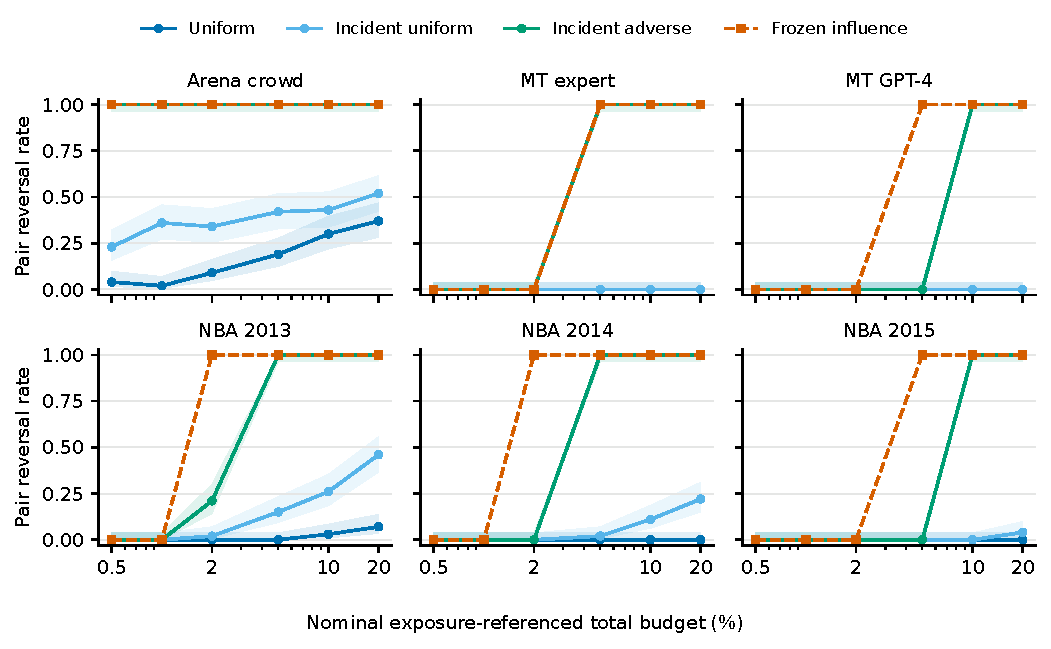
\includegraphics[width=\linewidth]{figures/dose_response.pdf}
\caption{Supplementary strict pair-reversal dose responses. Nominal fractions are $f\in\{0.005,0.01,0.02,0.05,0.1,0.2\}$ and actual integer budgets are $k=\max(1,\lceil fE_{ab}\rceil)$. The figure places points on the nominal grid, so plotted positions are not exact realized percentages after rounding. Random orderings are nested within a repeat, with 100 repeats; shaded bands are pointwise 95\% Wilson Monte Carlo intervals. Frozen influence has one deterministic ordering, not 100 replicates. Budgets exceeding an eligible ordering's length are omitted. Global controls can spend edits off-target, so the horizontal scale is exposure-referenced total cost, not always an incident-corruption fraction. Source: \texttt{artifacts/random\_curves.csv}; generated figure: \texttt{paper/figures/dose\_response.pdf}.}
\label{fig:dose}
\end{figure}

The dose-response grid is distinct from the primary powers-of-two witness search and its 20\%-of-decisive-rows cap. Secondary strict leader replacement is defined by $\max_j\theta_j>\theta_a+10^{-7}$. Secondary pair disagreement is the fraction of all unordered participant pairs whose fitted difference changes strict sign; pairs tied in either fit contribute zero. It is not a tie-corrected Kendall statistic. These metrics are logged in \texttt{random\_curves.csv}; no unsupported ranking-generalization claim is attached to them. The initial argmax-only winner-change metric could count ties; the corrected strict metric and its regression test supersede it.

\subsection{All adjacent baseline pairs}
\begin{figure}[htbp]
\centering
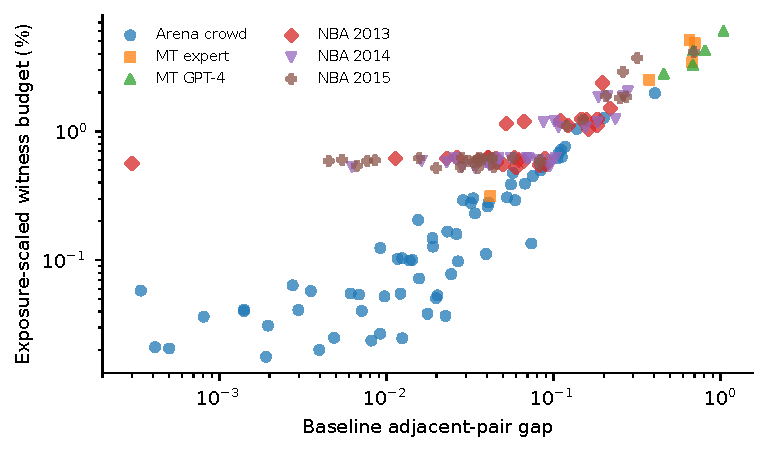
\includegraphics[width=0.85\linewidth]{figures/adjacent_pairs.pdf}
\caption{Secondary adjacent-pair audit: baseline gap versus exposure-scaled witness budget, both on logarithmic axes. The procedure audits \AdjacentCount{} adjacent pairs across the six baseline rankings. Points are selected-data descriptors; neither an association p-value nor a causal relationship is claimed. The same search incompleteness and denominator qualifications apply as for the primary audit. Source: \texttt{artifacts/adjacent.csv}; summaries: \texttt{artifacts/adjacent\_summary.csv}; generated figure: \texttt{paper/figures/adjacent\_pairs.pdf}.}
\label{fig:adjacent}
\end{figure}

The numbers of adjacent pairs follow the cohort sizes: 63 for Arena, five per MT release, and 29 per NBA season. Targets are selected from each baseline ordering; pair results share observations and are not independent tests. The CSV summaries include within-panel Spearman correlations as descriptive associations only. There is no selection-adjusted or multiplicity-corrected inferential claim for the most fragile pair, and the scatter is not evidence that gap alone determines edit budgets.

\section{Fixed-target estimator ablations}
\label{app:ablations}
\begin{table}[htbp]
\centering
\caption{Full fixed-target sensitivity results. Each row retains the corresponding primary target identities. The gap is before outcome edits under the changed estimator/data convention. $k=0$ with ``Already reversed'' means the specification change alone reverses the original pair, not a successful zero-edit attack on the primary specification. Other $k$ values are sufficient witnesses, not minima. Tie removal changes $N$ and $E_{ab}$; ridge alone does not. Source: \texttt{artifacts/fixed\_target\_ablations.csv}; generated input: \texttt{paper/tables/fixed\_ablations.tex}.}
\label{tab:ablations}
{\small\setlength{\tabcolsep}{4pt}\begin{tabular}{llrrl}
\toprule
Dataset & Change & Original-pair gap & $k$ & Status \\
\midrule
Arena crowd & $\lambda=0.1$ & 0.004 & 1 & Witness \\
Arena crowd & $\lambda=10$ & 0.044 & 11 & Witness \\
Arena crowd & Remove ties & -0.023 & 0 & Already reversed \\
MT expert & $\lambda=0.1$ & 0.378 & 46 & Witness \\
MT expert & $\lambda=10$ & 0.357 & 46 & Witness \\
MT expert & Remove ties & 0.527 & 42 & Witness \\
MT GPT-4 & $\lambda=0.1$ & 0.820 & 61 & Witness \\
MT GPT-4 & $\lambda=10$ & 0.724 & 61 & Witness \\
MT GPT-4 & Remove ties & 1.065 & 40 & Witness \\
MT GPT-4 & Remove inconsistent & 0.971 & 47 & Witness \\
NBA 2013 & $\lambda=0.1$ & 0.228 & 3 & Witness \\
NBA 2013 & $\lambda=10$ & 0.168 & 3 & Witness \\
NBA 2013 & Home covariate & 0.207 & 3 & Witness \\
NBA 2014 & $\lambda=0.1$ & 0.295 & 4 & Witness \\
NBA 2014 & $\lambda=10$ & 0.192 & 4 & Witness \\
NBA 2014 & Home covariate & 0.283 & 4 & Witness \\
NBA 2015 & $\lambda=0.1$ & 0.744 & 8 & Witness \\
NBA 2015 & $\lambda=10$ & 0.451 & 8 & Witness \\
NBA 2015 & Home covariate & 0.715 & 8 & Witness \\
\bottomrule
\end{tabular}
}
\end{table}

The primary $\lambda=1$ rows are in Table~\ref{tab:main}; Table~\ref{tab:ablations} supplies the changes around them. Ridge values 0.1 and 10 bracket the specified primary value without selecting a value for a preferred fragility result. On a sum loss, this is not a constant per-observation penalty across datasets or changing sample sizes. Removing all ties and excluding only GPT inconsistent rows test different conventions and have different denominators.

The earlier \texttt{artifacts/ablations.csv} reselects a leading pair after each change. That file is not used as evidence of same-target sensitivity. For example, reselecting the NBA 2015 runner-up can change both target identity and exposure; freezing identities avoids this conflation. A future result that is already reversed, numerically tied, or unresolved must keep that status rather than being replaced by a favorable newly selected pair. The present full fixed-target table includes the already-reversed Arena case explicitly.

\section{Adaptive flips and same-estimator deletion}
\label{app:comparators}
\begin{table}[htbp]
\centering
\caption{Supplementary method comparison on original targets. Adaptive flips refit and relinearize after every new edit; frozen flips use the initial ordering. Deletion removes rows under the same sum-loss ridge estimator. ``Linear prediction'' is the frozen first-order cumulative-budget prediction, not a verified finite edit result. Counts across interventions are not exchangeable and do not reproduce published deletion experiments. Sources: \texttt{artifacts/method\_comparison.csv} and \texttt{artifacts/baseline.csv}; generated input: \texttt{paper/tables/methods.tex}.}
\label{tab:methods}
{\small\begin{tabular}{lrrrr}
\toprule
Dataset & Frozen flips & Adaptive flips & Deletion & Linear prediction \\
\midrule
Arena crowd & 2 & 2 & 3 & 2 \\
MT expert & 46 & 46 & 92 & 45 \\
MT GPT-4 & 61 & 61 & 144 & 56 \\
NBA 2013 & 3 & 3 & 5 & 3 \\
NBA 2014 & 4 & 4 & 7 & 4 \\
NBA 2015 & 8 & 8 & 16 & 8 \\
\bottomrule
\end{tabular}
}
\end{table}

Adaptive selection recomputes flip benefits at each current optimum, chooses an available positive-benefit decisive row, never reuses a row, and refits the cumulative selected set against the original dataset. It uses the same target and decisive-row cap. The unchanged budgets in Table~\ref{tab:methods} provide no empirical improvement for this comparator on the six primary instances; neither procedure is an optimal solver.

For deletion, let $p_i$ be the original fitted probability. Infinitesimally removing row $i$ changes the margin by approximately $(p_i-y_i)c^\top H^{-1}x_i$, so the static harmful-deletion score is
\begin{equation}
 B_i^{\rm del}=-(p_i-y_i)x_i^\top H^{-1}c.
\label{eq:deletion}
\end{equation}
The implementation orders positive scores and searches deletion prefixes with full numerical refits, up to 20\% of original rows. Tie rows can have deletion influence even though they are ineligible for binary flips. Removal changes the comparison schedule and the likelihood information; a flip instead reverses an outcome while retaining its contribution to exposure. The penalty remains fixed in both procedures. Their count difference is an intervention comparison, not an efficiency ratio between algorithms and not a reproduction of \citet{huang2025dropping} or \citet{broderick2020automatic}. Their published snapshots, filtering choices, and estimators are not assumed to match ours.

\section{Reproduction instructions and artifact map}
\label{app:reproduction}
\subsection{Environment, commands, and measured resources}
The corrected main run records Python 3.11.15 on
\begin{quote}\small\path{Linux-7.0.0-38-generic-x86_64-with-glibc2.41}.\end{quote}
Dependencies used by the scripts include NumPy, pandas, SciPy, matplotlib, pyarrow, requests, and pytest. Numerical runs are CPU-only with \texttt{OPENBLAS\_NUM\_THREADS=1}, \texttt{OMP\_NUM\_THREADS=1}, and \texttt{MKL\_NUM\_THREADS=1}. The project's resource constraint was at most 8\,GB memory, at most 3\,GB data, and CPU-only operation; this is a constraint, not a measured peak-use claim. Visible CPU metadata and separately measured replay memory are reported below; visible host topology does not imply exclusive allocation.

The following commands reproduce the local-data path from the project root, here mounted at \texttt{/work}. They are documentation, not commands executed during manuscript drafting. Raw files must already exist at the four locations in \texttt{data/manifest.json} and match the listed hashes; these commands require no network access and do not infer new snapshots.
\begin{verbatim}
PYTHONPATH=/work/src python /work/src/prepare.py
OPENBLAS_NUM_THREADS=1 OMP_NUM_THREADS=1 MKL_NUM_THREADS=1 \
  PYTHONPATH=/work/src python -m pytest -q /work/tests
OPENBLAS_NUM_THREADS=1 OMP_NUM_THREADS=1 MKL_NUM_THREADS=1 \
  PYTHONPATH=/work/src python /work/src/run.py \
  --repeats 100 --bootstrap 200
OPENBLAS_NUM_THREADS=1 OMP_NUM_THREADS=1 MKL_NUM_THREADS=1 \
  PYTHONPATH=/work/src python /work/src/supplement.py
PYTHONPATH=/work/src python /work/src/report.py
\end{verbatim}
The last command regenerates tables, figures, \texttt{paper/numbers.tex}, and summary CSV/JSON files. It must follow the supplementary run because the report reads fixed-target ablations and comparator artifacts. The seven-test result in \texttt{artifacts/tests.log} is existing evidence, not a fresh test claimed by this writing pass. Script paths resolve their root from their own location rather than requiring a changed working directory.

\begin{table}[htbp]
\centering
\caption{Recorded per-dataset runtime instrumentation from the corrected main run. Fits count calls registered on each primary dataset's BT object; auxiliary bootstrap-pseudodataset, matching, and supplementary objects are not a complete project fit count. Seconds are measured per-dataset blocks, not hardware-normalized estimates. Gradient maxima are rounded. Source: \texttt{artifacts/runtime.csv}; generated input: \texttt{paper/tables/runtime.tex}.}
\label{tab:runtime}
{\small\begin{tabular}{lrrr}
\toprule
Dataset & Fits & Seconds & Max $\|g\|_\infty$ \\
\midrule
Arena crowd & 2691 & 17.77 & 1e-08 \\
MT expert & 2479 & 2.21 & 1e-08 \\
MT GPT-4 & 2481 & 2.41 & 9.8e-09 \\
NBA 2013 & 2455 & 3.96 & 1e-08 \\
NBA 2014 & 2458 & 4.02 & 9.9e-09 \\
NBA 2015 & 2468 & 4.21 & 9.5e-09 \\
\bottomrule
\end{tabular}
}
\end{table}

The corrected main script, including its ablation and matching stages, records \MainSeconds{} seconds elapsed. Table~\ref{tab:runtime} sums to \MainFitCount{} instrumented primary-object fit calls; its reported maximum gradient, rounded by the generator, is \texttt{\MaxGradient}. The separate supplement records approximately 3.46 seconds in \texttt{artifacts/supplement\_metadata.json}. Neither number includes all preparation, downloads, dependency installation, source reading, earlier failed or corrected runs, report rendering, or manuscript compilation. Total project compute was not fully metered; preliminary and failed runs are documented in \texttt{experiment\_log.md}. Dense Hessian storage scales quadratically and factorization cubically in participant count; the small cohorts here do not establish large-cohort scalability.

The visible CPU is an Intel Xeon Gold 6230 at 2.10\,GHz (\texttt{artifacts/hardware.txt}); the sequential numerical process uses one BLAS thread, not all visible host cores. A separately rooted replay in a newly created virtual environment installed \texttt{requirements.txt}: NumPy 2.4.6, SciPy 1.17.1, pandas 3.0.6, matplotlib 3.11.2, pyarrow 26.0.0, requests 2.34.2, pytest 9.2.0, pypdf 6.21.4, and threadpoolctl 3.7.0. Full transitive versions are in \texttt{artifacts/environment\_freeze.txt}. The replay's main run took 41.26 seconds and its child-process peak resident memory was 301.87\,MiB (Linux \texttt{resource.RUSAGE\_CHILDREN}; \texttt{artifacts/resource\_replay.json}). These measurements concern that replay only, not the complete project. All 13 deterministic result CSVs agree with the accepted run within $10^{-8}$ relative and $10^{-9}$ absolute tolerance; timing metadata is intentionally excluded. Seven tests also pass in the isolated environment. The replay shares checksummed raw files but runs relocated source code and a separately installed Python environment. It is not an independent data collection. A complete, copy-safe validation command from the project root is
\begin{verbatim}
PYTHONPATH=src python src/validate.py --replay reproduction_check
\end{verbatim}
The directory argument is the actual replay root; creation, installation, measurement and output comparison are documented in the accompanying README.

\subsection{Mapping reported outputs to source artifacts}
All tabular inputs and numerical figures are generated by \texttt{src/report.py}, not manually reconstructed in this manuscript. PDF and PNG figures with the same basename are available in \texttt{paper/figures/}.
\begin{itemize}
\item Table~\ref{tab:main}: \texttt{artifacts/baseline.csv} to \texttt{paper/tables/main.tex}; row-level evidence in \texttt{witness\_rows.csv} and \texttt{witness\_verification.csv}.
\item Figure~\ref{fig:budget}: \texttt{baseline.csv} and \texttt{uncertainty.csv} to \texttt{paper/figures/budget\_and\_margin.pdf}.
\item Table~\ref{tab:controls}: \texttt{controls.csv} to \texttt{control\_summary.csv} and \texttt{paper/tables/controls.tex}.
\item Table~\ref{tab:matched}: \texttt{matched.csv} to \texttt{matched\_summary.csv} and \texttt{paper/tables/matched.tex}; validation in \texttt{matching\_protocol.json}.
\item Table~\ref{tab:eda}: \texttt{eda.csv} to \texttt{paper/tables/eda.tex}.
\item Table~\ref{tab:bootstrap}: \texttt{uncertainty.csv} to \texttt{bootstrap\_summary.csv} and \texttt{paper/tables/bootstrap.tex}.
\item Figure~\ref{fig:dose}: \texttt{random\_curves.csv} to \texttt{paper/figures/dose\_response.pdf}.
\item Figure~\ref{fig:adjacent}: \texttt{adjacent.csv} to \texttt{adjacent\_summary.csv} and \texttt{paper/figures/adjacent\_pairs.pdf}.
\item Table~\ref{tab:ablations}: \texttt{fixed\_target\_ablations.csv} to \texttt{paper/tables/fixed\_ablations.tex}.
\item Table~\ref{tab:methods}: \texttt{method\_comparison.csv} and \texttt{baseline.csv} to \texttt{paper/tables/methods.tex}.
\item Table~\ref{tab:runtime}: \texttt{runtime.csv} to \texttt{paper/tables/runtime.tex}. \texttt{run\_metadata.json} also supplies \texttt{MainSeconds}; \texttt{numbers.tex} contains all five generated numerical macros used here.
\end{itemize}
Unless prefixed by \texttt{paper/}, the result basenames in this list reside under \texttt{artifacts/}. \texttt{src/bt.py} implements the estimator and finite verification; \texttt{src/prepare.py} specifies row units and mappings; \texttt{src/run.py} produces main comparisons; \texttt{src/supplement.py} produces fixed-target checks, adaptive/deletion comparisons, and original-row reconstruction. The pre-analysis plan and departures are preserved in \texttt{todos.md} and \texttt{experiment\_log.md}. A public hosting URL is not claimed; the complete code, pinned environment, generated numerical artifacts, and paper sources are supplied in the accompanying \texttt{reproducibility.zip}. Raw data remain separate. Original code is MIT-licensed; third-party datasets and the official template retain their own terms (\texttt{THIRD\_PARTY\_NOTICES.md}).

The paper was compiled with the official style unmodified; its main text ends on page seven, within the official nine-page limit. References, appendices, and the filled checklist are excluded from that content limit. The build command is
\begin{verbatim}
latexmk -pdf -interaction=nonstopmode -halt-on-error \
  -cd /work/paper/main.tex
\end{verbatim}
Style provenance and the official limit are recorded in \texttt{paper/template/PROVENANCE.md}. No fonts, margins, or official spacing were reduced for page compliance.

\section{Source boundaries, secondary-data ethics, and LLM disclosure}
\label{app:ethics}
\subsection{Literature scope and independence}
Only the five works in \texttt{paper/references.bib} are research-paper sources. Actual reading extents and pinned versions are logged in \texttt{artifacts/literature\_notes.md}; selected sections were read, not every proof or cited reference. We did not perform a broad search, follow citation graphs, or assert exhaustive novelty. No attempt was made to identify an unspecified prohibited work. Writing used local records only, without network access. Dataset locators and official template provenance are reproducibility assets rather than extra paper citations. Previously downloaded source bytes or a paper's bibliography do not imply that those cited works were consulted.

\subsection{No new human study; residual secondary-data obligations}
This audit recruits no participants, commissions no annotations, provides no participant-facing instructions, pays no new annotators, and runs no live manipulation. Its rows include previously released human preferences, so ``no new human study'' must not be confused with data having no human origin or ethical implications. We do not claim to have audited original consent, compensation, demographic representation, or all upstream collection practices. Original studies and asset owners remain the sources of those records.

Analysis requires participant/model IDs, outcomes, question/turn identifiers, and game covariates, not published prompt or answer examples. Processed edge lists omit prompt/answer text, and no raw dataset is bundled with the manuscript/code outputs. Public accessibility and a license do not by themselves eliminate privacy, consent, redistribution, or fairness obligations. We make no attempt to deanonymize judges or users and do not characterize a vulnerable row as a bad-faith or incorrect human annotation. Model rankings reflect the observed populations and conventions, not all users or protected groups.

No new institutional review approval or exemption is claimed. The supplied records do not include a formal institution-specific review determination for this secondary analysis, and we cannot certify legal or ethics-code compliance by inference. Formal NeurIPS Code of Ethics policy text was directly retrieved and reviewed during final verification (\texttt{artifacts/compliance/ethics\_readable.txt}), without following its further-reading links. The study avoids new participant interaction, minimizes redistributed data, attributes assets, communicates representativeness and dual-use limits, and supplies reproducibility artifacts. These steps address the policy relevant to this offline audit; they do not certify all upstream collection practices or supply an institution-specific determination.

\subsection{Benefits, harms, assets, and release status}
Potential benefits are more interpretable audit reports, reduced overconfidence in near-tied ranks, and identification of estimator conventions worth reporting. Potential harms include adapting influence selection to malicious voting, overstating offline access as a practical attack, or selectively presenting fragile ranks to discredit models or judges. Misinterpretation is possible even when the numerical procedure works as intended. The manuscript mitigates these risks by defining an offline threat model, disclosing access assumptions, distinguishing witnesses from minima, including negative controls and specification failures, and avoiding a label-correctness claim. None of these is a validated platform defense.

No new generative model, scraped corpus, or human-response dataset is released. The new products are audit scripts, aggregate results, witness row references, and manuscript artifacts. Recorded source licenses are Apache-2.0 for Arena and CC-BY-4.0 for MT/NBA; creators, snapshots, and hashes are given in Appendix~\ref{app:provenance}. The unchanged official template has its own provenance record. Original code and documentation are MIT-licensed, with exclusions for third-party assets. The accompanying anonymous archive includes complete code, pinned requirements, retained provenance and generated aggregates, but excludes raw data, source-paper PDFs, virtual environments, and replay copies. No public hosting URL or legal certification of every upstream practice is claimed. The pinned dataset READMEs and NBA license were directly reviewed; \texttt{THIRD\_PARTY\_NOTICES.md} records attribution, transformations and dependency-license information. Raw public data should remain separately obtained under original terms, not silently repackaged. No operational access to a live voting system is supplied.

\subsection{LLM assistance}
LLM-based assistants contributed to research planning, permitted-source synthesis, implementation assistance, local code/statistical auditing, experiment interpretation, and drafting/formatting this manuscript. Assistance was therefore broader than cosmetic prose editing. The numerical evidence comes from saved program outputs and independent original-row reconstruction, not from unverified generated numerical claims. Final verification included compilation, local mathematical/code review and an isolated-environment replay; no human independently approved the complete study. The GPT-4 judgments analyzed in MT-Bench are pre-existing exported data; no new paid model API calls or generated judging labels were used for this audit. Exact assistant model/version metadata is not established by the supplied artifacts, and no claim of independent human validation of the full draft is made.

\clearpage
\section*{NeurIPS Paper Checklist}

% Official NeurIPS 2026 questions and guidelines retained; instruction block removed.
% Answers reflect the final verified local release and supplied anonymous archive.
\begin{enumerate}

\item {\bf Claims}
    \item[] Question: Do the main claims made in the abstract and introduction accurately reflect the paper's contributions and scope?
    \item[] Answer: \answerYes{}
    \item[] Justification: Sections~\ref{sec:introduction}--\ref{sec:sensitivity} identify the results as fixed-schedule, estimator-conditional witness upper bounds and report controls and specification failures. Neither novelty priority, minimum-budget certification, production-ranking replication, nor causal design/judge effects are claimed.
    \item[] Guidelines:
    \begin{itemize}
        \item The answer \answerNA{} means that the abstract and introduction do not include the claims made in the paper.
        \item The abstract and/or introduction should clearly state the claims made, including the contributions made in the paper and important assumptions and limitations. A \answerNo{} or \answerNA{} answer to this question will not be perceived well by the reviewers. 
        \item The claims made should match theoretical and experimental results, and reflect how much the results can be expected to generalize to other settings. 
        \item It is fine to include aspirational goals as motivation as long as it is clear that these goals are not attained by the paper. 
    \end{itemize}

\item {\bf Limitations}
    \item[] Question: Does the paper discuss the limitations of the work performed by the authors?
    \item[] Answer: \answerYes{}
    \item[] Justification: Section~\ref{sec:discussion} and Appendices~\ref{app:matching}--\ref{app:ethics} discuss near ties, ridge/tie conventions, incomplete search, dependence, selected-target uncertainty, confounded comparisons, access assumptions, incomplete metering of total project compute, and unverified upstream collection practices. The Arena tie-removal reversal and the unchanged adaptive budgets are retained as limiting or negative results.
    \item[] Guidelines:
    \begin{itemize}
        \item The answer \answerNA{} means that the paper has no limitation while the answer \answerNo{} means that the paper has limitations, but those are not discussed in the paper. 
        \item The authors are encouraged to create a separate ``Limitations'' section in their paper.
        \item The paper should point out any strong assumptions and how robust the results are to violations of these assumptions (e.g., independence assumptions, noiseless settings, model well-specification, asymptotic approximations only holding locally). The authors should reflect on how these assumptions might be violated in practice and what the implications would be.
        \item The authors should reflect on the scope of the claims made, e.g., if the approach was only tested on a few datasets or with a few runs. In general, empirical results often depend on implicit assumptions, which should be articulated.
        \item The authors should reflect on the factors that influence the performance of the approach. For example, a facial recognition algorithm may perform poorly when image resolution is low or images are taken in low lighting. Or a speech-to-text system might not be used reliably to provide closed captions for online lectures because it fails to handle technical jargon.
        \item The authors should discuss the computational efficiency of the proposed algorithms and how they scale with dataset size.
        \item If applicable, the authors should discuss possible limitations of their approach to address problems of privacy and fairness.
        \item While the authors might fear that complete honesty about limitations might be used by reviewers as grounds for rejection, a worse outcome might be that reviewers discover limitations that aren't acknowledged in the paper. The authors should use their best judgment and recognize that individual actions in favor of transparency play an important role in developing norms that preserve the integrity of the community. Reviewers will be specifically instructed to not penalize honesty concerning limitations.
    \end{itemize}

\item {\bf Theory assumptions and proofs}
    \item[] Question: For each theoretical result, does the paper provide the full set of assumptions and a complete (and correct) proof?
    \item[] Answer: \answerYes{}
    \item[] Justification: The paper claims no novel theoretical result or finite-edit approximation bound; Appendix~\ref{app:derivation} states the finite-design and positive-ridge assumptions and derives existence, uniqueness, centering, aggregation, and the implicit derivative used in the method. The derivative is explicitly not a finite-flip guarantee or optimality certificate.
    \item[] Guidelines:
    \begin{itemize}
        \item The answer \answerNA{} means that the paper does not include theoretical results. 
        \item All the theorems, formulas, and proofs in the paper should be numbered and cross-referenced.
        \item All assumptions should be clearly stated or referenced in the statement of any theorems.
        \item The proofs can either appear in the main paper or the supplemental material, but if they appear in the supplemental material, the authors are encouraged to provide a short proof sketch to provide intuition. 
        \item Inversely, any informal proof provided in the core of the paper should be complemented by formal proofs provided in appendix or supplemental material.
        \item Theorems and Lemmas that the proof relies upon should be properly referenced. 
    \end{itemize}

    \item {\bf Experimental result reproducibility}
    \item[] Question: Does the paper fully disclose all the information needed to reproduce the main experimental results of the paper to the extent that it affects the main claims and/or conclusions of the paper (regardless of whether the code and data are provided or not)?
    \item[] Answer: \answerYes{}
    \item[] Justification: Sections~\ref{sec:method}--\ref{sec:data} and Appendices~\ref{app:data}--\ref{app:reproduction} specify the objective, snapshots/hashes, edit units, targets, search, seeds, controls, resampling, and exact local commands with script/artifact mappings. Package versions are pinned, seven tests pass, original-row witnesses are independently reconstructed, and a newly installed isolated-environment replay agrees on 13 deterministic result CSVs (Appendix~\ref{app:reproduction}).
    \item[] Guidelines:
    \begin{itemize}
        \item The answer \answerNA{} means that the paper does not include experiments.
        \item If the paper includes experiments, a \answerNo{} answer to this question will not be perceived well by the reviewers: Making the paper reproducible is important, regardless of whether the code and data are provided or not.
        \item If the contribution is a dataset and\slash or model, the authors should describe the steps taken to make their results reproducible or verifiable. 
        \item Depending on the contribution, reproducibility can be accomplished in various ways. For example, if the contribution is a novel architecture, describing the architecture fully might suffice, or if the contribution is a specific model and empirical evaluation, it may be necessary to either make it possible for others to replicate the model with the same dataset, or provide access to the model. In general. releasing code and data is often one good way to accomplish this, but reproducibility can also be provided via detailed instructions for how to replicate the results, access to a hosted model (e.g., in the case of a large language model), releasing of a model checkpoint, or other means that are appropriate to the research performed.
        \item While NeurIPS does not require releasing code, the conference does require all submissions to provide some reasonable avenue for reproducibility, which may depend on the nature of the contribution. For example
        \begin{enumerate}
            \item If the contribution is primarily a new algorithm, the paper should make it clear how to reproduce that algorithm.
            \item If the contribution is primarily a new model architecture, the paper should describe the architecture clearly and fully.
            \item If the contribution is a new model (e.g., a large language model), then there should either be a way to access this model for reproducing the results or a way to reproduce the model (e.g., with an open-source dataset or instructions for how to construct the dataset).
            \item We recognize that reproducibility may be tricky in some cases, in which case authors are welcome to describe the particular way they provide for reproducibility. In the case of closed-source models, it may be that access to the model is limited in some way (e.g., to registered users), but it should be possible for other researchers to have some path to reproducing or verifying the results.
        \end{enumerate}
    \end{itemize}

\item {\bf Open access to data and code}
    \item[] Question: Does the paper provide open access to the data and code, with sufficient instructions to faithfully reproduce the main experimental results, as described in supplemental material?
    \item[] Answer: \answerYes{}
    \item[] Justification: The accompanying anonymous \texttt{reproducibility.zip} supplies all code, pinned requirements, generated results and instructions; public raw datasets are downloaded separately at fixed URLs with checksums. Appendices~\ref{app:provenance} and \ref{app:reproduction} give sources, seeds, commands and the table/figure mapping. No publicly hosted code URL or bundled raw data is claimed.
    \item[] Guidelines:
    \begin{itemize}
        \item The answer \answerNA{} means that paper does not include experiments requiring code.
        \item Please see the NeurIPS code and data submission guidelines (\url{https://neurips.cc/public/guides/CodeSubmissionPolicy}) for more details.
        \item While we encourage the release of code and data, we understand that this might not be possible, so \answerNo{} is an acceptable answer. Papers cannot be rejected simply for not including code, unless this is central to the contribution (e.g., for a new open-source benchmark).
        \item The instructions should contain the exact command and environment needed to run to reproduce the results. See the NeurIPS code and data submission guidelines (\url{https://neurips.cc/public/guides/CodeSubmissionPolicy}) for more details.
        \item The authors should provide instructions on data access and preparation, including how to access the raw data, preprocessed data, intermediate data, and generated data, etc.
        \item The authors should provide scripts to reproduce all experimental results for the new proposed method and baselines. If only a subset of experiments are reproducible, they should state which ones are omitted from the script and why.
        \item At submission time, to preserve anonymity, the authors should release anonymized versions (if applicable).
        \item Providing as much information as possible in supplemental material (appended to the paper) is recommended, but including URLs to data and code is permitted.
    \end{itemize}

\item {\bf Experimental setting/details}
    \item[] Question: Does the paper specify all the training and test details (e.g., data splits, hyperparameters, how they were chosen, type of optimizer) necessary to understand the results?
    \item[] Answer: \answerYes{}
    \item[] Justification: Sections~\ref{sec:estimator}--\ref{sec:data} give the all-observed-row evaluation protocol, specified sum-loss ridge, tie mapping, optimizer tolerances, edit cap, and strict reversal endpoint; no supervised split or predictive-generalization claim is invented. Appendices~\ref{app:derivation}, \ref{app:matching}, and \ref{app:uncertainty} detail aggregation, seeds, matching, and resampling departures from the initial plan.
    \item[] Guidelines:
    \begin{itemize}
        \item The answer \answerNA{} means that the paper does not include experiments.
        \item The experimental setting should be presented in the core of the paper to a level of detail that is necessary to appreciate the results and make sense of them.
        \item The full details can be provided either with the code, in appendix, or as supplemental material.
    \end{itemize}

\item {\bf Experiment statistical significance}
    \item[] Question: Does the paper report error bars suitably and correctly defined or other appropriate information about the statistical significance of the experiments?
    \item[] Answer: \answerYes{}
    \item[] Justification: Section~\ref{sec:controls} and Appendix~\ref{app:uncertainty} define two-sided pointwise Wilson Monte Carlo intervals, selected-target empirical percentile bands, and seed ranges, distinguishing each source of variability. No simultaneous, post-selection-valid, minimum-budget, or multiplicity-controlled significance claim is made; deterministic witnesses are conditional evidence rather than population tests.
    \item[] Guidelines:
    \begin{itemize}
        \item The answer \answerNA{} means that the paper does not include experiments.
        \item The authors should answer \answerYes{} if the results are accompanied by error bars, confidence intervals, or statistical significance tests, at least for the experiments that support the main claims of the paper.
        \item The factors of variability that the error bars are capturing should be clearly stated (for example, train/test split, initialization, random drawing of some parameter, or overall run with given experimental conditions).
        \item The method for calculating the error bars should be explained (closed form formula, call to a library function, bootstrap, etc.)
        \item The assumptions made should be given (e.g., Normally distributed errors).
        \item It should be clear whether the error bar is the standard deviation or the standard error of the mean.
        \item It is OK to report 1-sigma error bars, but one should state it. The authors should preferably report a 2-sigma error bar than state that they have a 96\% CI, if the hypothesis of Normality of errors is not verified.
        \item For asymmetric distributions, the authors should be careful not to show in tables or figures symmetric error bars that would yield results that are out of range (e.g., negative error rates).
        \item If error bars are reported in tables or plots, the authors should explain in the text how they were calculated and reference the corresponding figures or tables in the text.
    \end{itemize}

\item {\bf Experiments compute resources}
    \item[] Question: For each experiment, does the paper provide sufficient information on the computer resources (type of compute workers, memory, time of execution) needed to reproduce the experiments?
    \item[] Answer: \answerYes{}
    \item[] Justification: Appendix~\ref{app:reproduction} reports the visible Xeon Gold 6230 CPU, single-thread numerical execution, pinned Python environment, per-dataset main runtime and measured isolated replay (41.26 seconds, 301.87 MiB peak RSS). Preliminary, corrected and failed runs are disclosed; exact total project compute was not fully metered. No GPU or model training was used.
    \item[] Guidelines:
    \begin{itemize}
        \item The answer \answerNA{} means that the paper does not include experiments.
        \item The paper should indicate the type of compute workers CPU or GPU, internal cluster, or cloud provider, including relevant memory and storage.
        \item The paper should provide the amount of compute required for each of the individual experimental runs as well as estimate the total compute. 
        \item The paper should disclose whether the full research project required more compute than the experiments reported in the paper (e.g., preliminary or failed experiments that didn't make it into the paper). 
    \end{itemize}

\item {\bf Code of ethics}
    \item[] Question: Does the research conducted in the paper conform, in every respect, with the NeurIPS Code of Ethics \url{https://neurips.cc/public/EthicsGuidelines}?
    \item[] Answer: \answerYes{}
    \item[] Justification: The official policy was directly retrieved and reviewed during final verification. Section~\ref{sec:discussion} and Appendix~\ref{app:ethics} address no new participant interaction, privacy-minimizing secondary use, attribution, nonrepresentativeness, dual-use risks and reproducibility. No live system was manipulated, institutional approval fabricated, or all-upstream compliance certification claimed; the policy access and asset notices are retained.
    \item[] Guidelines:
    \begin{itemize}
        \item The answer \answerNA{} means that the authors have not reviewed the NeurIPS Code of Ethics.
        \item If the authors answer \answerNo, they should explain the special circumstances that require a deviation from the Code of Ethics.
        \item The authors should make sure to preserve anonymity (e.g., if there is a special consideration due to laws or regulations in their jurisdiction).
    \end{itemize}

\item {\bf Broader impacts}
    \item[] Question: Does the paper discuss both potential positive societal impacts and negative societal impacts of the work performed?
    \item[] Answer: \answerYes{}
    \item[] Justification: Section~\ref{sec:discussion} and Appendix~\ref{app:ethics} describe transparent audit communication as a benefit and manipulation, misleading rank presentation, privacy, and representativeness risks as potential harms. Offline scope and conservative claim boundaries are disclosure safeguards, not experimentally validated platform defenses.
    \item[] Guidelines:
    \begin{itemize}
        \item The answer \answerNA{} means that there is no societal impact of the work performed.
        \item If the authors answer \answerNA{} or \answerNo, they should explain why their work has no societal impact or why the paper does not address societal impact.
        \item Examples of negative societal impacts include potential malicious or unintended uses (e.g., disinformation, generating fake profiles, surveillance), fairness considerations (e.g., deployment of technologies that could make decisions that unfairly impact specific groups), privacy considerations, and security considerations.
        \item The conference expects that many papers will be foundational research and not tied to particular applications, let alone deployments. However, if there is a direct path to any negative applications, the authors should point it out. For example, it is legitimate to point out that an improvement in the quality of generative models could be used to generate Deepfakes for disinformation. On the other hand, it is not needed to point out that a generic algorithm for optimizing neural networks could enable people to train models that generate Deepfakes faster.
        \item The authors should consider possible harms that could arise when the technology is being used as intended and functioning correctly, harms that could arise when the technology is being used as intended but gives incorrect results, and harms following from (intentional or unintentional) misuse of the technology.
        \item If there are negative societal impacts, the authors could also discuss possible mitigation strategies (e.g., gated release of models, providing defenses in addition to attacks, mechanisms for monitoring misuse, mechanisms to monitor how a system learns from feedback over time, improving the efficiency and accessibility of ML).
    \end{itemize}

\item {\bf Safeguards}
    \item[] Question: Does the paper describe safeguards that have been put in place for responsible release of data or models that have a high risk for misuse (e.g., pre-trained language models, image generators, or scraped datasets)?
    \item[] Answer: \answerNA{}
    \item[] Justification: No new pretrained model, scraped corpus, or raw human-response dataset is released; outputs are offline audit artifacts and row references, as stated in Appendix~\ref{app:ethics}. Dual-use manipulation risks are discussed explicitly, but no high-risk generative asset or validated technical defense is claimed.
    \item[] Guidelines:
    \begin{itemize}
        \item The answer \answerNA{} means that the paper poses no such risks.
        \item Released models that have a high risk for misuse or dual-use should be released with necessary safeguards to allow for controlled use of the model, for example by requiring that users adhere to usage guidelines or restrictions to access the model or implementing safety filters. 
        \item Datasets that have been scraped from the Internet could pose safety risks. The authors should describe how they avoided releasing unsafe images.
        \item We recognize that providing effective safeguards is challenging, and many papers do not require this, but we encourage authors to take this into account and make a best faith effort.
    \end{itemize}

\item {\bf Licenses for existing assets}
    \item[] Question: Are the creators or original owners of assets (e.g., code, data, models), used in the paper, properly credited and are the license and terms of use explicitly mentioned and properly respected?
    \item[] Answer: \answerYes{}
    \item[] Justification: Appendix~\ref{app:provenance} and \texttt{THIRD\_PARTY\_NOTICES.md} credit dataset owners and associated papers, identify fixed versions and reviewed Apache-2.0/CC-BY-4.0 terms, document transformations, and exclude raw data from redistribution. Official template provenance/headers are preserved and dependencies are installed, not vendored. No legal certification of every upstream collection practice is asserted.
    \item[] Guidelines:
    \begin{itemize}
        \item The answer \answerNA{} means that the paper does not use existing assets.
        \item The authors should cite the original paper that produced the code package or dataset.
        \item The authors should state which version of the asset is used and, if possible, include a URL.
        \item The name of the license (e.g., CC-BY 4.0) should be included for each asset.
        \item For scraped data from a particular source (e.g., website), the copyright and terms of service of that source should be provided.
        \item If assets are released, the license, copyright information, and terms of use in the package should be provided. For popular datasets, \url{paperswithcode.com/datasets} has curated licenses for some datasets. Their licensing guide can help determine the license of a dataset.
        \item For existing datasets that are re-packaged, both the original license and the license of the derived asset (if it has changed) should be provided.
        \item If this information is not available online, the authors are encouraged to reach out to the asset's creators.
    \end{itemize}

\item {\bf New assets}
    \item[] Question: Are new assets introduced in the paper well documented and is the documentation provided alongside the assets?
    \item[] Answer: \answerYes{}
    \item[] Justification: The anonymous accompanying archive contains MIT-licensed audit code, tests, pinned requirements, full reproduction instructions, numerical outputs, manuscript sources and provenance. Appendix~\ref{app:reproduction} and the README map every table/figure to its generating script. Limitations, units, seeds and reuse boundaries are documented; no new human labels, raw conversations or model are released.
    \item[] Guidelines:
    \begin{itemize}
        \item The answer \answerNA{} means that the paper does not release new assets.
        \item Researchers should communicate the details of the dataset\slash code\slash model as part of their submissions via structured templates. This includes details about training, license, limitations, etc. 
        \item The paper should discuss whether and how consent was obtained from people whose asset is used.
        \item At submission time, remember to anonymize your assets (if applicable). You can either create an anonymized URL or include an anonymized zip file.
    \end{itemize}

\item {\bf Crowdsourcing and research with human subjects}
    \item[] Question: For crowdsourcing experiments and research with human subjects, does the paper include the full text of instructions given to participants and screenshots, if applicable, as well as details about compensation (if any)? 
    \item[] Answer: \answerNA{}
    \item[] Justification: This study recruits no participants and commissions no crowdsourcing or new judgments; it reanalyzes public secondary data (Appendix~\ref{app:ethics}). Original participant instructions, compensation, and consent are not newly asserted or audited, and the lack of new recruitment does not eliminate secondary-data obligations.
    \item[] Guidelines:
    \begin{itemize}
        \item The answer \answerNA{} means that the paper does not involve crowdsourcing nor research with human subjects.
        \item Including this information in the supplemental material is fine, but if the main contribution of the paper involves human subjects, then as much detail as possible should be included in the main paper. 
        \item According to the NeurIPS Code of Ethics, workers involved in data collection, curation, or other labor should be paid at least the minimum wage in the country of the data collector. 
    \end{itemize}

\item {\bf Institutional review board (IRB) approvals or equivalent for research with human subjects}
    \item[] Question: Does the paper describe potential risks incurred by study participants, whether such risks were disclosed to the subjects, and whether Institutional Review Board (IRB) approvals (or an equivalent approval/review based on the requirements of your country or institution) were obtained?
    \item[] Answer: \answerNA{}
    \item[] Justification: There is no new participant interaction or human-subject experiment in this offline secondary analysis, and no new IRB approval or exemption is claimed. Appendix~\ref{app:ethics} discusses residual privacy/consent risks and explicitly states that an institution-specific review determination and upstream collection compliance were not established by the supplied evidence.
    \item[] Guidelines:
    \begin{itemize}
        \item The answer \answerNA{} means that the paper does not involve crowdsourcing nor research with human subjects.
        \item Depending on the country in which research is conducted, IRB approval (or equivalent) may be required for any human subjects research. If you obtained IRB approval, you should clearly state this in the paper. 
        \item We recognize that the procedures for this may vary significantly between institutions and locations, and we expect authors to adhere to the NeurIPS Code of Ethics and the guidelines for their institution. 
        \item For initial submissions, do not include any information that would break anonymity (if applicable), such as the institution conducting the review.
    \end{itemize}

\item {\bf Declaration of LLM usage}
    \item[] Question: Does the paper describe the usage of LLMs if it is an important, original, or non-standard component of the core methods in this research? Note that if the LLM is used only for writing, editing, or formatting purposes and does \emph{not} impact the core methodology, scientific rigor, or originality of the research, declaration is not required.
    %this research? 
    \item[] Answer: \answerYes{}
    \item[] Justification: Appendix~\ref{app:ethics} discloses LLM assistance in planning, source synthesis, implementation, auditing, interpretation, and manuscript preparation, not just editing, and distinguishes assistance from the saved numerical evidence. The MT GPT-4 labels are pre-existing exported results; no new judging API calls were made, and exact assistant model/version metadata is not invented.
    \item[] Guidelines:
    \begin{itemize}
        \item The answer \answerNA{} means that the core method development in this research does not involve LLMs as any important, original, or non-standard components.
        \item Please refer to our LLM policy in the NeurIPS handbook for what should or should not be described.
    \end{itemize}

\end{enumerate}

\end{document}
